\documentclass[output=paper]{LSP/langsci}
\author{Ekaterina Lapshinova-Koltunski}
\title{Variation in translation: Evidence from corpora}
%\epigram{Change epigram in chapters/01.tex or remove it there}
\abstract{The present paper describes a corpus-based approach to study variation in translation in terms of translation features. We compare texts, which differ in the source/target texts (English vs. German), production types (original vs. translation) and method of translation (human, computer-aided = \textsc{cat}, machine) in terms of a theoretically-motivated set of features. In this study, we decide for the features which can be easily obtained on the basis of automatic corpus annotations, i.e. tokens, lemmas and part-of-speech tags. Our results show that there is variation in the mentioned translations in terms of the features under analysis.}
\maketitle

\begin{document}

\section{Introduction: Aims and Motivation} \label{sec:4:1}

In this paper, we apply corpus-based methods to analyse translation variants – translations from English into German produced with different translation methods.

Although numerous studies on translation operate with corpus-based methods, most of them concentrate on the questions concerning the nature of translations and their specific features, \citep[see e.g.][]{Baker1993,Baker1995,Laviosa2002,Chesterman2004} and others. The majority of them tried to generalise translation by defining certain rules or regularities of translated texts.  Moreover, they mostly compare translations with originals, i.e. differences or similarities between translations and their source texts or comparable non-translated texts, ignoring variation which can be observed in different translation variants. Corpus-based studies dedicated to the analysis of variation phenomena involving translations, \citep[e.g.][]{Teich2003,Steiner2004,Neumann2013}, etc. concentrate on the analysis of human translations only. However, nowadays, translations are produced not only by humans but also with machine translation (MT) systems. Furthermore, new variants of translation appear due to the interaction of both, e.g. in computer-aided translation or post-editing.

In some works on machine translation the focus lies on comparing different translation variants, such as human vs. machine, as in  \citep{White1994,Papineni2002,BabychHartley2004,Popovic2011}. However, they all serve the task of automatic MT system evaluation and use the human-produced translations as references or training material only. None of them provide an analysis of specific linguistically motivated features of different text types translated with different translation methods, which is the aim of the present analysis.

In this study, we aim to apply corpus-based methods to prove the knowledge of translation features on a new dataset which contains different variants of translations, including human and machine translation.

The remainder of the paper is structured as follows. \sectref{sec:4:2} presents studies we adopt as theoretical background for the selection of features under analysis. In \sectref{sec:4:3:1}, we describe the resources and methods used. In \sectref{sec:4:4}, we present the results of our analyses and their discussion, and in \sectref{sec:4:5}, we draw some conclusions and provide more ideas for future work.

\section{Theoretical Background} \label{sec:4:2}

Since the present study concentrates on the analysis of linguistic features of different translation variants, we address the existing studies on translation for their definition.

\subsection{Related Feature Work}

As already mentioned in \sectref{sec:4:1} above, in most cases, these studies either analyse differences between original texts and translations \citep{House1997,Matthiessen2001,Teich2003,Hansen2003,Steiner2004}, or concentrate on the properties of translated texts only \citep{Baker1995}. Nevertheless, an important point is that most of them consider translations to have their own specific properties which distinguish them from the originals: both their source texts and comparable texts in the target language. These features establish the specific language of translations which is called \textit{translationese} defined by \citep{Gellerstam1986}. Comparing Swedish translations from English with Swedish original texts, the author stated significant differences between them, whereas not all of them were attributable to the source language. This coincides with what \citet{Frawley1984} called 'third code’, describing features of translational language which are supposed to be different from both source and target languages.

Later, Mona Baker emphasised general effects of the process of translation that are independent of source language, e.g. in \citet{Baker1993,Baker1995}. Analysing characteristic patterns of translations, she excluded the influence of the source language on a translation altogether. Within this context, she proposed \textit{translation universals} – linguistic features which typically occur in translated rather than original texts. According to \citet{Baker1993}, they are independent of the influence of the specific language pairs involved in the process of translation. Other scholars (e.g. \citealt{Toury1995} or \citealt{Chesterman2004}) operate with other terms – \textit{laws} or \textit{regularities}. We prefer to use the term \textit{translation features} or \textit{phenomena} in the present study: to claim the features 'universal’ we would need to analyse more language pairs and translation directions, and to call them 'laws’ and 'regularities’, we would need to test more conditions, e.g. cognitive factors, status of translation, etc., which is not possible with the bilingual dataset at hand.

Translation features can be classified according to different parameters. For instance, \citet{Chesterman2004} makes a distinction between \textit{S-universals} and \textit{T-universals}: the first comprises differences between translations and their source texts, and the second covers the differences between translations and comparable non-translated texts. A more fine-grained classification includes the following features: \textit{explicitation} – tendency to spell things out rather than leave them implicit, \textit{simplification} – tendency to simplify the language used in translation, \textit{normalisation} – a tendency to exaggerate features of the target language and to conform to its typical patterns, \textit{levelling out}– individual translated texts are more alike than individual original texts, in both source and target languages, and \textit{interference} – features of the source texts are observed in translations. For the second last, we prefer the term convergence proposed by \citet{Laviosa2002}, which implies a relatively higher level of homogeneity of translated texts with regard to their own scores on given measures of universal features, e.g. lexical density, sentence length, etc. in contrast to originals.  For the last feature, we also prefer to use the term “\textit{shining through}” defined by \citet{Teich2003}.

All these features have been widely analysed in corpus-based translation studies for different language pairs, e.g. in \citet{Laviosa1996} for English translations from a variety of source languages, in \citet{Mauranen2000} for English-Finnish translations, in \citet{Teich2003} for English and German translations, and others. Yet, all of them concentrate on human translations only.

Moreover, some recent corpus-based studies applied machine learning supervised methods to automatically differentiate between translations and originals \citep[e.g.][]{Baroni2006}. These approaches found application in some recent works on natural language processing, e.g. those on cleaning parallel corpora obtained from the Web, or improvement of translation and language models in MT  \citep[e.g.][]{Kurokawa2009,KoppelOrdan2011,Lembersky2012}.

We employ the knowledge from these studies, as well as techniques applied to explore the differences between translation variants under analysis, including the features related to their source texts as well as those of comparable target texts.

\subsection{Translation Features and their Operationalisation} \label{sec:4:2:2}

We group the features described above into three classes according to their correlations, especially in their operationalisation: 1) simplification, 2) explicitation, 3) normalisation vs. “shining though” and 4) convergence. Simplification can be analysed on different levels, e.g. lexical, syntactic or semantic. If core patterns of lexical use are observed, \citep[see][]{Laviosa1998}, we can identify simplification comparing the proportion of content vs. grammatical words. Translated texts have a relatively low percentage of content words, and the most frequent words are repeated more often. This means, that both lexical density and type-token-ratio of translations is lower than those of their source texts and the comparable texts in the target language.  Besides, more general terms are expected to be used in translations.  On the level of syntax, one can observe short sentences which replace long ones and a lower average sentence length in general.

Explicitation involves the addition and specification of lexical and grammatical items, with the help of which implicit information in the source text is “spelled out” in its translation.  The indicators of this feature include a higher ratio of function words which make grammatical relations explicit, specific terms replacing more general terms (the opposite of simplification), disambiguation of pronouns, increased use of cohesive devices, e.g. conjunctions, and others. In terms of cohesion, one would also expect more nominal (expressed with nominal phrases) than pronominal reference (expressed with personal pronouns) in translations.

Simplification and explicitation features correlate and may be just the opposite of each other.  For example, if we observe more specific terms replacing general terms in translation, we face the feature of explicitation, and not simplification. Normalisation and “shining through” can also be measured on different levels, depending on the languages involved. Both features depend on the contrasts between these languages: normalisation implies the exaggerated use of the patterns typical for the target languages, whereas “shining through” involves the patterns typical for the source language (but not specific for the target language) that can be observed in translations. For instance, normalisation can be verified by a great number of typical collocations and neutralised metaphoric expressions. \citet{Baker1996} claims that influence of normalisation depends on the status of the source language: “the higher the status of the source text and language, the less the tendency to normalise”. We assume that the languages with a higher status also tend to “shine through” more often. For example, if we analyse translations from English, we would probably observe more “shining through” than normalisation, as English has the highest world language status.

And finally, convergence is a homogeneity feature of translations:  they reveal less variation if we compare them to original texts.  Convergence can also be observed on all levels of a language system. In accordance with the convergence phenomenon, one would expect that the lexical, grammatical and syntactic features under analysis will reveal smaller differences in translations than in originals.

\subsection{Hypotheses} \label{sec:4:2:3}

For our analysis of translation variants, we select a set of operationalisation of the features described in \sectref{sec:4:2:2} above. 
 
\begin{enumerate}
\item \textbf{Simplification} - We expect that our translated texts have a lower percentage of content words vs. grammatical words than their English source texts and the comparable German texts. Also, words are repeated more often in translations. Thus, we observe lower lexical density and type-token-ratio in our translations. In the analysis of English to German translations, we exclude sentence length as operationalisation for simplification. Due to the systemic differences in the morphology, German sentences are generally shorter than those in English, as they contain one-word compounds. To measure this uniformly, we need to split compounds and measure their parts as tokens, which is not feasible within this study.

\item \textbf{Explicitation} - Our translated texts reveal more cohesive explicitness than English and German originals: we can observe more conjunctions, less pronominal reference and less general nouns in translations than in English and German originals.

\item \textbf{Normalisation}/ \textbf{“shining through”} - If the translations under analysis demonstrate features more typical for English than for German, we observe “shining through”. If there are more features typical for German originals, then our translations demonstrate normalisation. Here, we use the knowledge from contrastive analysis, e.g. German-English contrasts described in \citep{Hawkins1986,KoenigGast2007,Steiner2012}. For example, we know that English is more “verbal” than German. This can be proved by comparing the distribution of nominal and verbal phrases in both translations and originals. English originals are expected to contain more verbal than nominal phrases. The phenomenon of “shining through” will be confirmed in our data if translations contain more verbal phrases than German originals. On the contrary, it they contain less verbal phrases than German originals, the normalisation hypothesis will be confirmed.

\item \textbf{Convergence} - The variation of the features in 1) to 3) is not great if we compare translation variants: they are similar to each other, i.e. the features are distributed homogeneously.
\end{enumerate}

\section{Resources, Methods and Tools} \label{sec:4:3}

To prove the hypotheses formulated in \sectref{sec:4:2:3}, we need to compare the distribution of the features under analysis across translation variants, their English sources as well as comparable German originals. For this, we analyse frequency distribution information of lexico-grammatical patterns which serve as operationalisation for these features. The patterns are extracted from a corpus at hand, and evaluated with univariate statistical methods (e.g. significance analysis).

\subsection{Corpus Resources} \label{sec:4:3:1}
For our investigations, we use \textsc{vartra}-\textsc{small}, \citep[see][]{Lapshinova2013}, a translation corpus which contains German translation variants from English produced with different translation methods: by (1) human professionals (PT), (2) human inexperienced translators (\textsc{cat}), with (3) rule-based MT systems (RBMT) and (4) two statistical MT systems (SMT1 and SMT2). Translations by professionals (PT) were exported from the already existing corpus CroCo \citep{HansenSchirra2013}. The same corpus provides source English texts (EO) and comparable German originals (GO). Thus, we can compare source English texts with their multiple translations into German, as well as to comparable German originals.

The \textsc{cat} variant was produced by trained translators with at least BA degree, who have no/little experience in translation. All of them applied computer-aided tools while translating the given texts\footnote{We used the open source tool ACROSS, see \url{www.my-across.net}}. The rule-based machine translation variant was translated with SY\textsc{st}RAN (RBMT)\footnote{SY\textsc{st}RAN 6}, whereas for statistical machine translation we have two further versions – the one produced with Google Translate\footnote{\url{http://translate.google.com/}} (SMT1), and the other – with a self-trained Moses system (SMT2) \citep[see][]{Hoang2007}.

The analysed dataset covers seven registers of written language: political \textsc{essay}s (\textsc{essay}), fictional texts (\textsc{fiction}), manuals (\textsc{instr}), popular-scientific articles (\textsc{popsci}), “letters to share-holders” (\textsc{share}), prepared political speeches (\textsc{speech}), and tourism leaflets (TOU).The size of all translation variants in \textsc{vartra}-\textsc{small} comprises approx. 600 thousand tokens.  The subcorpora of originals from CroCo comprise around 250 thousand words each.

All subcorpora under analysis are tokenised, lemmatised and tagged with part-of-speech information, segmented into syntactic chunks and sentences.  The annotations of the \textsc{vartra}-\textsc{small} subcorpora were obtained with Tree Tagger \citep{Schmid1994}. The availability of these annotation levels in both corpora allows us to analyse certain lexico-grammatical patterns – operationalisation of the translation features under analysis, defined in \sectref{sec:4:2:3}.

The subcorpora are encoded in CWB format (CWB, 2010) and can be queried with the help of the CQP regular expressions described in \citep{Evert2005}.

Alignment on sentence level is available for professional translations only: each translation is aligned with its English source on sentence level.  No alignment is provided for further translation variants at the moment. However, this annotation level is not necessary for the extraction of the operationalization used in the present paper.

\subsection{Feature Extraction}
As already mentioned in \sectref{sec:4:3:1} above, the corpus at hand can be queried with CQP, which allows the definition of language patterns in form of regular expressions based on string, part-of-speech and chunk tags as well as further constraints.

To prove the hypothesis for simplification indicated by lexical density (proportion of content words), we extract information on the distribution of content words in our corpus, for which the query 1 in \tabref{tab:4.1} is used.

To extract the corpus evidence of explicitation, we apply queries 2 to 5. Query 2 is used to extract all occurrences of coordinating and subordinating conjunctions, whereas queries 3 and 4 are used for extraction of information on pronominal vs. nominal reference in the corpus. 

\begin{table}
     \centering
     \begin{tabular}{lll}
\lsptoprule
              & \textbf{query element}         & \textbf{explanation} \\ \midrule
\textbf{1}    & [pos=”VV.*|N.*|\textsc{adj}.*|ADV”]     & a full verb/noun or an adjective/adverb \\
\textbf{2}    & [pos=”KON|KOUS”]               & connector or subordinator \\
\textbf{3}    & <NP>[pos=”PPE.*”]+</NP>		   & nominal phrase filled with a pronoun \\
\textbf{4}    & <NP>[ ]+</NP>             & any nominal phrase \\ 
\textbf{5}    & [lemma=RE(\$general)]     & nouns from a list   \\ 
\textbf{6}    & (<NP>[]+</NP>)|(<PP>[]+</PP>) & nominal phrase or prepositional phrase \\
\textbf{7}    & <VP>[]+</VP> & verbal phrase\\
\lspbottomrule
     \end{tabular}

 \caption{Queries for feature extraction}
     \label{tab:4.1}
     % Verweis im Text mittels \REF{tbl:beispieltabelle}
\end{table}

We calculate this as proportion of nominal phrases filled with personal pronouns (query 3) to all nominal phrases in the corpus (query 4). Query 5 is used to extract occurrences of general terms in order to compare their proportion to all nouns in the dataset. For this, we use a simple lexical search – we extract a closed class of lexical items of which we know the members. Here, we use lists of general nouns as defined in \citep{Dipper2012}. For normalisation/“shining through”, we extract all occurrences of nominal and prepositional phrases (query 6) vs. verbal phrases (query 7). Convergence is proved with the help of all patterns described above.

As we operate with low-level features which do not require formulation of complex lexico-grammatical patterns, we believe that our feature extraction procedures are adequate for the present task.  Its only shortcoming is the potential noise caused by tagging errors, especially in case of machine translation. In the latter, we observe a number of untranslated words which are tagged as named entities by automatic part-of-speech taggers.  In the longer run, we aim to include deeper structures into our analysis which would require parsed data.

\section{Results and their Interpretation} \label{sec:4:4} 
\subsection{Simplification}
In the first step, we want to test if lexical density and type-token-ratio are lower in translation variant than in EO and GO.


     \begin{table}
     \centering
     \resizebox{\textwidth}{!}{
     \begin{tabular}{llllllll}
     \lsptoprule
              & \textbf{EO}  & \textbf{GO} & \textbf{PT	\textsc{cat}} & \textbf{HU-$\bar{x}$} & \textbf{RBMT	SMT1	SMT2} & \textbf{MT-$\bar{x}$}  & \textbf{Trans-$\bar{x}$}\\ \midrule 
\textbf{LD}    & \textbf{45.72 }    & \textbf{45.49} & 46.23	44.60  & \textbf{45.64} & 45.08	46.02	47.86 & \textbf{46.30} & \textbf{45.97} \\
\textbf{\textsc{st}TR}  & \textbf{367.5}    & \textbf{369.9} & 360.8	336.4  & \textbf{348.6} & 335.2	350.4	309.0 & \textbf{331.5} & \textbf{338.4} \\
\lspbottomrule
\end{tabular}
}
 \caption{\textsc{st}TR and LD in \textsc{vartra}-\textsc{small}}
     \label{tab:4.2}
% Verweis im Text mittels \REF{tbl:beispieltabelle}
\end{table}


As already mentioned above, lexical density (LD in \tabref{tab:4.2}) is measured as a proportion of all content words in our corpus. Unexpectedly, average lexical density in translations (Trans-$\bar{x}$ in \tabref{tab:4.2}) does not differ from that of both source and comparable originals. Moreover, if we consider the mean values for human and machine translations separately (HU-$\bar{x}$ and MT-$\bar{x}$ respectively); the latter demonstrates even higher LD than human translations and English and German originals. The lowest figure is obtained for \textsc{cat}, which demonstrates a value below the average. The highest value is observed for SMT2 (47.86).

We explain this by the lexical constraints of the Moses-based system: this system depends on the parallel data used for its training.  If the parallel data does not contain translations for some words in a text to be translated, the system keeps them untranslated. In the automatic part-of-speech tagging, these words are then tagged as proper nouns (NE) which leads to their high amount in texts, as seen in example \REF{ex:4:1}.

However, the overall difference between originals and translations is not great, which means that lexical density is not an indicator of simplification in our dataset, as the translated texts show an amount of content words similar to that of the source and comparable originals.

\ea \label{ex:4:1}
Wenn/KOUS Sie/PPER strongly/NE ,/\$, believe/NE ,/\$, wie/KOKOM ich/PPER ,/\$, dass/KOUS Großbritannien/NE einen/\textsc{art} zentralen/\textsc{adja} Platz/NN einnehmen/VVINF müssen/VMINF in/APPR Europe’s/NE decision-making/NE...
\z

Another indicator of simplification is type-token-ratio which we measure as standardised type-token-ratio (\textsc{st}TR) – a percentage of different lexical word forms (types) per text.  As expected, on average, translations show lower \textsc{st}TR than their source texts and comparable originals, see \tabref{tab:4.2}. Mean value of human translations is also higher than that of machine (348.6 vs. 338.6 respectively). Within translations, the highest \textsc{st}TR, thus, the most lexically rich translation variant in our corpus, is the one produced by professional human translators (360.8), followed by SMT1 (350.4), and \textsc{cat} (336.4).  The level of the latter is close to the average of all translations but lower than that of human translations. The lowest figure is obtained for SMT2 (309.0). This can once again be explained by the fact that this translation variant contains a great deal of untranslated English words, the lemmas of which cannot be identified by the lemmatiser and thus is replaced with '<unknown>’, see example \REF{ex:4:2}.

\ea \label{ex:4:2}
Closing/<\textit{unknown}> die/d Gap/<\textit{unknown}> Zwischen/zwischen \textit{Supply}/<\textit{unknown}> und/und Die/d Nachfrage/Nachfrage nach/nach A/A \textit{balanced}/<\textit{unknown}> ,/, umfassende/umfassend Energiepolitik/Energiepolitik ist/sein dringend/dringend erforderlich/  erforderlich ,/, die/d langfristige/langfristig Stärke/Stärke der/d  amerikanische/amerikanisch wirtschaftlichen/wirtschaftlich und/und nationalen/national <\textit{unknown}>.
\z

Interestingly, student translations are closer to the RBMT translation variant in terms of both \textsc{st}TR (336.4 vs. 335.2) and LD (44.60 vs. 45.08). Analysing human and machine translation separately, we observe the same ranking in terms of both indicators: PT > \textsc{cat}, whereas it is not stable in machine translation: while SMT2 ranks first in LD, it occupies the last position with its \textsc{st}TR value.

\subsection{Explicitation}

To analyse this feature in our corpus, we measure cohesive explicitness in all subcorpora. Here, we calculate the relative frequencies for conjunctions (conj in \tabref{tab:4.3}, normalised to the total number of words per thousand), proportion of nominal phrases filled with pro-forms vs. full nominal phrases (pronNP in \tabref{tab:4.3}, normalised per thousand), as well as proportion of general nouns vs. all noun occurrences (gennoun in \tabref{tab:4.3} normalised per thousand) in translations and English and German originals.

\begin{table}
     \centering
     \begin{tabular}{llll}
\lsptoprule
              & \textbf{conj}         & \textbf{pronNP}  & \textbf{gennoun} \\ \midrule
\textbf{EO}    & \textbf{53.80}     & \textbf{204.67} & \textbf{48.71} \\ 
\textbf{GO}    & \textbf{43.58}     & \textbf{127.14} & \textbf{23.85} \\ 
\textbf{PT}    & 47.58		        & 232.76          & 19.64 \\
\textbf{\textsc{cat}}   & 49.67		        & 139.12          & 19.93  \\ 
\textbf{HU-$\bar{x}$}    & \textbf{48.33}     & \textbf{184.67}   & \textbf{19.74}\\ 
\textbf{RBMT}  & 53.32		        & 144.46          & 23.18 \\
\textbf{SMT1}  & 52.54		        & 143.15          & 21.22 \\
\textbf{SMT2}  & 53.69		        & 39.85           & 19.46 \\ 
\textbf{MT-$\bar{x}$} & \textbf{53.18}  & \textbf{107.65}  & \textbf{21.19} \\ 
\textbf{Trans-$\bar{x}$} & \textbf{50.76}  & \textbf{137.76}  & \textbf{20.51} \\ 
\lspbottomrule
     \end{tabular}

 \caption{Explicitation indicators}
     \label{tab:4.3}
     % Verweis im Text mittels \REF{tbl:beispieltabelle}
\end{table}

According to our hypothesis in \sectref{sec:4:2:3}, we expect more conjunctions, less pronominal reference and less general nouns in translations than in originals. If we compare the values of all translations (Trans-$\bar{x}$) with those of their originals, our hypothesis can be confirmed for pronominal reference and general nouns only: Trans-$\bar{x}$ (137.76) < EO (204.67) and Trans-$\bar{x}$ (20.51) < EO (48.71). Translations demonstrate a lower and not higher distribution of conjunctions, Trans-$\bar{x}$ (50.67) < EO (53.80), contrary to what was expected. If we consider human and machine translation separately, we see that values for machine translation are much closer to EO (53.18 vs. 53.80), which means that in these translation variants, cohesive relation expressed via conjunctions, were preserved similarly to their English originals. Conversely, fewer conjunctions were used in human translation. The number is still higher than observed in German originals (43.58); therefore, we cannot assume the phenomenon of normalization here. This means that, in our dataset, human translators tend to keep that relation implicit, as seen in example \REF{ex:4:3}.


%\ea
%\ea Negative molecules moved into the nurse cells if the egg was made negative, while positive molecules stayed put (EO-\textsc{popsci}).
%\ex Wenn das Ei auch negativ war, bewegten sich negativ geladene Moleküle in die Nährzellen, positiv geladene Moleküle blieben an Ort und Stelle (PT-\textsc{popsci}).
%\z
%\z

\ea \label{ex:4:3}
\ea Negative molecules moved into the nurse cells if the egg was made negative, while positive molecules stayed put (EO-\textsc{popsci}).
\ex Wenn das Ei auch negativ war, bewegten sich negativ geladene Moleküle in die Nährzellen, positiv geladene Moleküle blieben an Ort und Stelle (PT-\textsc{popsci}).
\z
\z

Admittedly, our extractions exclude occurrences of adverbial conjunctions (as we extract coordinating and subordinating conjunctions only). Previous analyses \citep[e.g.][]{KunzLapshinova2014} show that this syntactic type of conjunction is highly frequent in German. We suppose that English coordinating and subordinating conjunctions are in some cases translated with adverbials in German. 

Example \REF{ex:4:4} extracted from our corpus demonstrates variants of translation of the English subordinating conjunction 'while'. In both human translations (b. and c.), conjunctive relation is transferred with an adverbial phrase. In machine translated variants (d. to f.), 'while' is translated directly with \textit{während}, so the type of cohesive conjunction is preserved as it was in the original.

\ea \label{ex:4:4}
\ea And \textit{while} this will vary from quarter to quarter based on large cash outlays such as tax payments and end-of-year compensation payments, we were pleased with our average positive cash flow for the year from operations of \$ 1.5 billion per quarter. (EO-\textsc{share}).
\ex Dieser Wert schwankt bei Betrachtung verschiedener Quartale. Dafür sind Auszahlungen hoher Beträge (z.B. Steuerzahlungen) sowie Ausgleichszahlungen am Jahresende verantwortlich. Mit dem durchschnittlichen operativen Cashflow von 1,5 Milliarden US-Dollar pro Quartal sind wir \textit{jedoch} höchst zufrieden (PT-\textsc{share}).
\ex  Dieser Cash Flow fällt zwar aufgrund von hohen Barauslagen, wie Steuern und Ausgleichszahlungen am Jahresende, in jedem Quartal unterschiedlich aus, \textit{dennoch} waren wir mit unserem durchschnittlichen jährlichen Cash Flow aus laufenden Geschäftstätigkeiten von 1,5 Millionen \$ pro Quartal zufrieden (\textsc{cat}-\textsc{share}).
\ex  Und basiert \textit{während} dieses von Viertel zu das Viertel schwankt, das auf grossen Barauslagen wie Steuerzahlungen und Jahresendeausgleichszahlungen, wurden wir mit unserem durchschnittlichen positiven Cashflow für das Jahr von den Operationen von \$1,5 Milliarde pro Viertel gefallen (RBMT-\textsc{share}).
\ex  Und \textit{während} dies von Quartal zu Quartal basierend auf grosse Barauslagen wie Steuer-Zahlungen und End-of-Jahres-Ausgleichszahlungen variieren, wurden wir mit unserer durchschnittlichen positiven Cashflow für das Jahr aus dem operativen Geschäft von 1,5 Milliarden Dollar pro Quartal (SMT1-\textsc{share}).
\ex  Und \textit{während} diese je nach Viertel bis Viertel auf der Grundlage grosse Geld ausgegeben wie Steuerzahlungen und abschliessende Entschädigung payments, freuen wir uns mit unseren durchschnittliche positive Cashflow für das Jahr von Maßnahmen der \$1.5 Milliarden pro quarter (SMT2-\textsc{share}).
\z
\z

In some cases, cohesion might be expressed with different cohesive devices in the two languages under analysis. For instance, the conjunction 'while' in the source sentence in example \REF{ex:4:5} is substituted with a reference expressed with the pronominal adverb \textit{dabei} in PT, see (\ref{ex:4:5}-b). Pronominal adverbs expressing a reference are typical for German and are rare in English. At the same time, we observe the adoption of the cohesive device used in the source sentence also in other translation variants (c. to f.).

\ea \label{ex:4:5}
\ea My father preferred to stay in a bathrobe and be waited on for a change \textit{while} he lead the stacks of newspapers me and my grandmother saved for him (EO-\textsc{fiction}).
\ex Mein Vater ist lieber im Bademantel geblieben und hat sich zur Abwechslung mal bedienen lassen und \textit{dabei} die Zeitungsstapel durchgelesen, die ich und meine Großmutter für ihn aufgehoben haben (PT-\textsc{fiction}).
\ex Mein Vater saß die ganze Zeit im Bademantel da und ließ sich zur Abwechslung bedienen, \textit{während} er die Zeitungen laß, die meine Großmutter und ich für ihn aufgehoben hatten (\textsc{cat}-\textsc{fiction}).
\ex Mein Vater bevorzugt, um in einem Bademantel zu bleiben und auf eine Änderung, \textit{während} er die Stapel von Zeitungen ich und meine führt Großmutter an gewartet zu werden gerettet für ihn (RBMT-\textsc{fiction}). 
\ex Mein Vater lieber im Bademantel bleiben und werden wartete auf eine Veränderung, \textit{während} er die Stapel von Zeitungen mich und meine Großmutter für ihn gerettet führen (SMT1-\textsc{fiction}).
\ex My Vater lieber Aufenthalt in einem bathrobe und gewartet werden über einen Klimawandel, während er die Stapeln kramen Zeitungen für mich und meine Großmutter him (SMT2-\textsc{fiction}).
\z
\z

In terms of reference, translations demonstrate less noun phrases filled with pronouns than their source texts in English: 137.76 (Trans-$\bar{x}$) vs. 204.14 (EO), whereas the opposite phenomenon is observed, if we compare them to the original texts in German. In this case, we observe more pronominal reference in translations than in comparable originals (137.76 vs. 127.14). However, variation is observed across translation variants: while in human translations pronominal reference is much higher and tends to the values of EO, machine translation shows values which are lower when compared to both EO and GO. This low value is obviously caused by the small amount of pronominal phrases in SMT2. Here, we suppose that many pronouns remained untranslated in certain registers, as seen in example (\ref{ex:4:5}-f) above, and were wrongly tagged in the part-of-speech annotation. Moreover, we observe a high number of pronominal references in PT (232.76), which contradicts the hypothesis in \sectref{sec:4:2:3}.

The figures obtained for general nouns confirm our hypothesis about their low frequency in translations. On average, translations demonstrate a lower amount of general nouns than EO and GO (20.51 vs. 48.71 and 23.85 respectively). RBMT is the only translation variant whose distribution of general nouns is similar to that of GO. As seen from the values for the originals, there are more general nouns in EO than in GO. This means that this type of nouns is more typical for English than for German. Hence, we observe normalisation in terms of general nouns in all translation variants of our corpus. 

In the analysis of explicitation in translations from English into German, one should also take into account the fact that German is more explicit than English, which could also have the influenced on the results obtained.

\subsubsection{Normalisation and “shining through”}
 
To analyse normalisation and “shining through”, we extracted all occurrences of nominal and prepositional phrases and compared them with the occurrences of verbal phrases. \tabref{tab:4.4} demonstrates the proportions of nominal (nominal and prepositional phrases) and verbal (verbal phrases) classes across all subcorpora under analysis. As already mentioned in \sectref{sec:4:2:3} above, German is less “verbal” than English, which is confirmed in our data: GO contains less verbal phrases than EO.

The mean value of verbal phrases for all translations comprises 28.63, which is much lower than that of GO. This indicates the phenomenon of normalisation in this case. Comparing the values across translation variants, we observe variation in the degree of normalisation – it is less pronounced in human than in machine translation (33.59 vs. 24.64 respectively).  Moreover, human translations produced by professionals are very close to German originals in terms of the distribution of nominal vs. verbal phrases, which means that they demonstrate neither normalisation nor “shining through” if we consider the indicators under analysis.

The higher noun-verb-ratio (NVratio in \tabref{tab:4.4}) is observed for SMT2. The reason for it could once again be the erroneous part-of-speech tagging which results from the gaps in training data used for SMT2. Most untranslated verbs (e.g. promote, report, import) or verbal forms (recognising, closing, helping, etc.) were tagged as nouns or adjectives.


\begin{table}
     \centering
     \begin{tabular}{llll}
\lsptoprule
\textbf{subc}    & \textbf{nominal}  & \textbf{verbal}  & \textbf{NVratio} \\ \midrule
\textbf{EO}    & 59.45   & 40.55  & 1.47 \\ \midrule
\textbf{GO}    & 61.95   & 38.05  & 1.63 \\ \midrule
\textbf{PT}    & 61.92	 & 38.08  & 1.63 \\
\textbf{\textsc{cat}}   & 71.87   & 28.13  & 2.56  \\ \midrule
\textbf{HU-$\bar{x}$}   & 66.41  & 33.59   & 1.98\\ \midrule
\textbf{RBMT}  & 72.42   & 27.58  & 2.63 \\
\textbf{SMT1}  & 74.38	 & 25.62  & 2.90 \\
\textbf{SMT2}  & 79.54   & 20.46  & 3.89 \\ \midrule
\textbf{MT-\textit{x}}   & 75.35  & 24.64  & 3.06 \\ \midrule
\textbf{Trans-$\bar{x}$} & 71.36 & 28.63  & 2.49 \\ 
\lspbottomrule
     \end{tabular}

 \caption{Proportionality of nominal vs. verbal opposition in \textsc{vartra}-\textsc{small}}
     \label{tab:4.4}
     % Verweis im Text mittels \REF{tbl:beispieltabelle}
\end{table}


Overall, the results are surprising rather than expected. Analysing examples in our corpus, we notice that source verbal phrases in human translations from English into German are often translated as nominal phrases, see examples (\ref{ex:4:6}-a), (\ref{ex:4:6}-b) and (\ref{ex:4:6}-c). However, they are often left as verbal phrases in machine translation, as in examples (\ref{ex:4:6}-d), (\ref{ex:4:6}-e) and (\ref{ex:4:6}-f). Therefore, we would expect machine-produced translations to have a lower noun-verb-ratio, which is not the case in the quantitative data.  To analyse the correspondences between source and target phrases we need to align our subcorpora, which is not available at the moment.

\ea \label{ex:4:6}
\ea Settings \textit{changed} here override settings \textit{changed} anywhere else (EO-\textsc{instr}).
\ex Die hier vorgenommenen \textit{Änderungen} setzen alle anderen \textit{Änderungen} außer Kraft (PT\textsc{instr}).
\ex Hier vorgenommene Einstellungs\textit{änderungen} sind allen anderen Einstellungs\textit{änderungen} übergeordnet (\textsc{cat}-\textsc{instr}).
\ex Die Einstellungen, die hier \textit{geändert} werden, heben die Einstellungen auf, die irgendwoanders \textit{geändert} werden (RBMT-\textsc{instr}).
\ex Hier \textit{geänderten} Einstellungen überschreiben Einstellungen, die anderswo \textit{geändert} (SMT1-\textsc{instr}).
\ex ... bei dem Sie überhaupt hier über Rahmenbedingungen \textit{geändert} Settings überall else (SMT2-\textsc{instr}).
\z
\z

\subsection{Convergence}

In our last hypothesis, we test if the analysed translations exhibit convergence – the variation of the features across translation variants in our corpus is not high. For this purpose, we consider the indicators analysed in \sectref{sec:4:1}, \sectref{sec:4:2} and \sectref{sec:4:3} above: \textsc{st}TR, LD, conj, pronNP, gennoun and NVratio. The overall variation between the subcorpora is relatively low for all features, except for pronominal reference and noun-verb-ratio (see \figref{fig:4:1}), which means that translation variants in our corpus are alike in terms of the features considered.  Most prominent indicators for convergence are that of simplification.  We remove pronominal reference and noun-verb-ratio from the data matrix and calculate p-values using the Pearson’s chi-square test, which is a univariate statistical method to reveal significant differences between variables. If p-value is < 0.05, then the difference between the compared subcorpora (translation variants) is not significant.

\begin{figure}
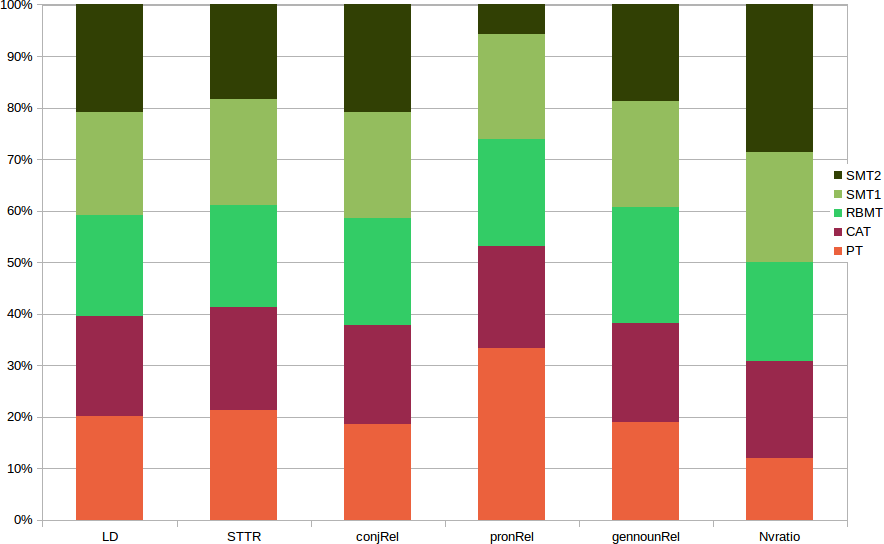
\includegraphics[width=1.0\textwidth]{./figures/5-1.png}
\caption{Levelling out in \textsc{vartra}-\textsc{small}} \label{fig:4:1}
\end{figure} 

\begin{table}
     \centering
     \begin{tabular}{lll}
          \lsptoprule
               & \textbf{subc}    & \textbf{p-value}  \\ \midrule
\textbf{PT}	   & vs. \textsc{cat}   & 0.8863     \\ 
	  	       & vs. RBMT  & 0.5663      \\ 
		       & vs. SMT1  & 0.8806       \\
		       & vs. SMT2  & 0.0142        \\ \midrule
\textbf{\textsc{cat}}   & vs. RBMT  & 0.9307         \\ 
			   & vs. SMT1  & 0.9986  		 \\
			   & vs. SMT2  & 0.0980           \\ \midrule
\textbf{RBMT}  & vs. SMT1  & 0.9373            \\ 
			   & vs. SMT2  & 0.1771			    \\ \midrule
\textbf{SMT1}  & vs. SMT2  & 0.0731 	         \\ 
\lspbottomrule
     \end{tabular}

 \caption{p-values for comparison of translation variants}
     \label{tab:4.5}
     % Verweis im Text mittels \REF{tbl:beispieltabelle}
\end{table}   

We calculate p-value for all pairs of subcorpora in \textbf{\textsc{vartra}}. The results confirm our assumptions, as p-value is above 0.05 in almost all cases (see \tabref{tab:4.5}). An exception is pair \textbf{PT-SMT2}, where we observe a p-value of approx. 0.01. Our translation variants therefore converge, as expected, as there is no significant difference between almost all subcorpora; they are alike in terms of the analysed phenomena, which are indicators of simplification, explicitation and normalisation.

\subsection{Summary}

Summarising the obtained results, we found that not all hypotheses formulated in \sectref{sec:4:2:3} above can be applied to our dataset. Both type-token-ratio as well as lexical density do not serve as good indicators of simplification in this case. In terms of explicitation, we should also think of further operationalisation, as those chosen reveal rather other phenomena (e.g. normalisation).  The hypotheses about normalisation and “shining through” can be confirmed only in part and reflect high variations across translation varieties.  The only assumption confirmed by our data is that of convergence.  The analysed translation variants converge, as there is no significant difference between them in terms of the analysed phenomena.

\section{Conclusion and Future Work} \label{sec:4:5}

In this paper, we analysed translation variants produced by humans and machine systems and compared them to their English source texts, as well as comparable German originals. With the help of lexicogrammatical patterns, we were able to trace differences and similarities between them, which indicate the following translation features: simplification, explicitation, normalisation and convergence. Although our analysis includes translations from English into German, we could not detect “shining through” - at least with the indicators at hand. The analysed features vary if we consider translation variants or their groups separately, e.g. in terms of explicitation or normalisation. At the same time, we observe convergence in translation, especially if we take simplification into account.

We believe that we should include more factors into the analysis to explain the variation observed. For example, in some cases, we should revise our hypotheses and their operationalisation, as contrasts between languages should be taken into account. We also need to look at the “experience” factor – this could verify the differences between two human translations observed for some features. Furthermore, restrictions of the translation memory applied in \textsc{cat} or the training material used in SMT can also have an influence on the distribution of lexico-grammatical patterns. For this, a closer inspection of correlations between translation memory as well as applied SMT training material (parallel corpora) is required, which is planned for our future work.

We also plan to align originals with their translations on word and sentence level to allow analysis of certain phenomena involved, e.g. translation of ambiguous cases, direct translation solutions, see 4.3 and their multiple variants.

\section*{Acknowledgments}
The project “\textsc{vartra}: Translation Variation” was supported by a grant from Forschungsausschuss of the Saarland University.


\printbibliography[heading=subbibliography,notkeyword=this]

\end{document}